\chapter{Statistical Thermodynamics Applied}\label{ch:b3:statistical-thermo-applied}

Liquid hydrogen kept in the best insulated tank still boils away, and in the
first days after liquefaction it boils away far faster than the heat leaking
through the walls can explain. The heat comes from inside the liquid. Hydrogen
molecules exist in two forms, which differ only in the relative orientation of
the spins of their two protons and which convert into one another only very
slowly; at \qty{20}{K} the conversion of one form into the other releases more
heat than is needed to evaporate the liquid. This chapter applies the
partition functions of \cref{ch:b3:partition-functions} to heat capacities, to
these nuclear-spin isomers and to the entropy that some crystals keep at 0 K,
then computes equilibrium constants and isotope effects from spectroscopic
data alone.

\begin{recall}
\Cref{ch:b3:partition-functions} built the \omterm{def:b3:partition-functions:partition-function}{molecular partition function} and its
four factors, and derived $U$, $S$ and $G$ from it. The Year 2 volume related
the standard equilibrium constant to the standard Gibbs energy of reaction,
$\Delta_rG^\circ = -RT\ln K^\circ$, and established the van 't Hoff equation;
\cref{ch:b3:many-electron-atoms} stated that a wavefunction changes sign when two
identical fermions are exchanged; \cref{ch:b3:rovibrational-spectroscopy} found
the 3:1 alternation of line intensities in the rotational Raman spectrum of
\ce{H2}-like molecules. The Grade 9 part of the first volume defined isotopes.
\end{recall}

\begin{omfigure}
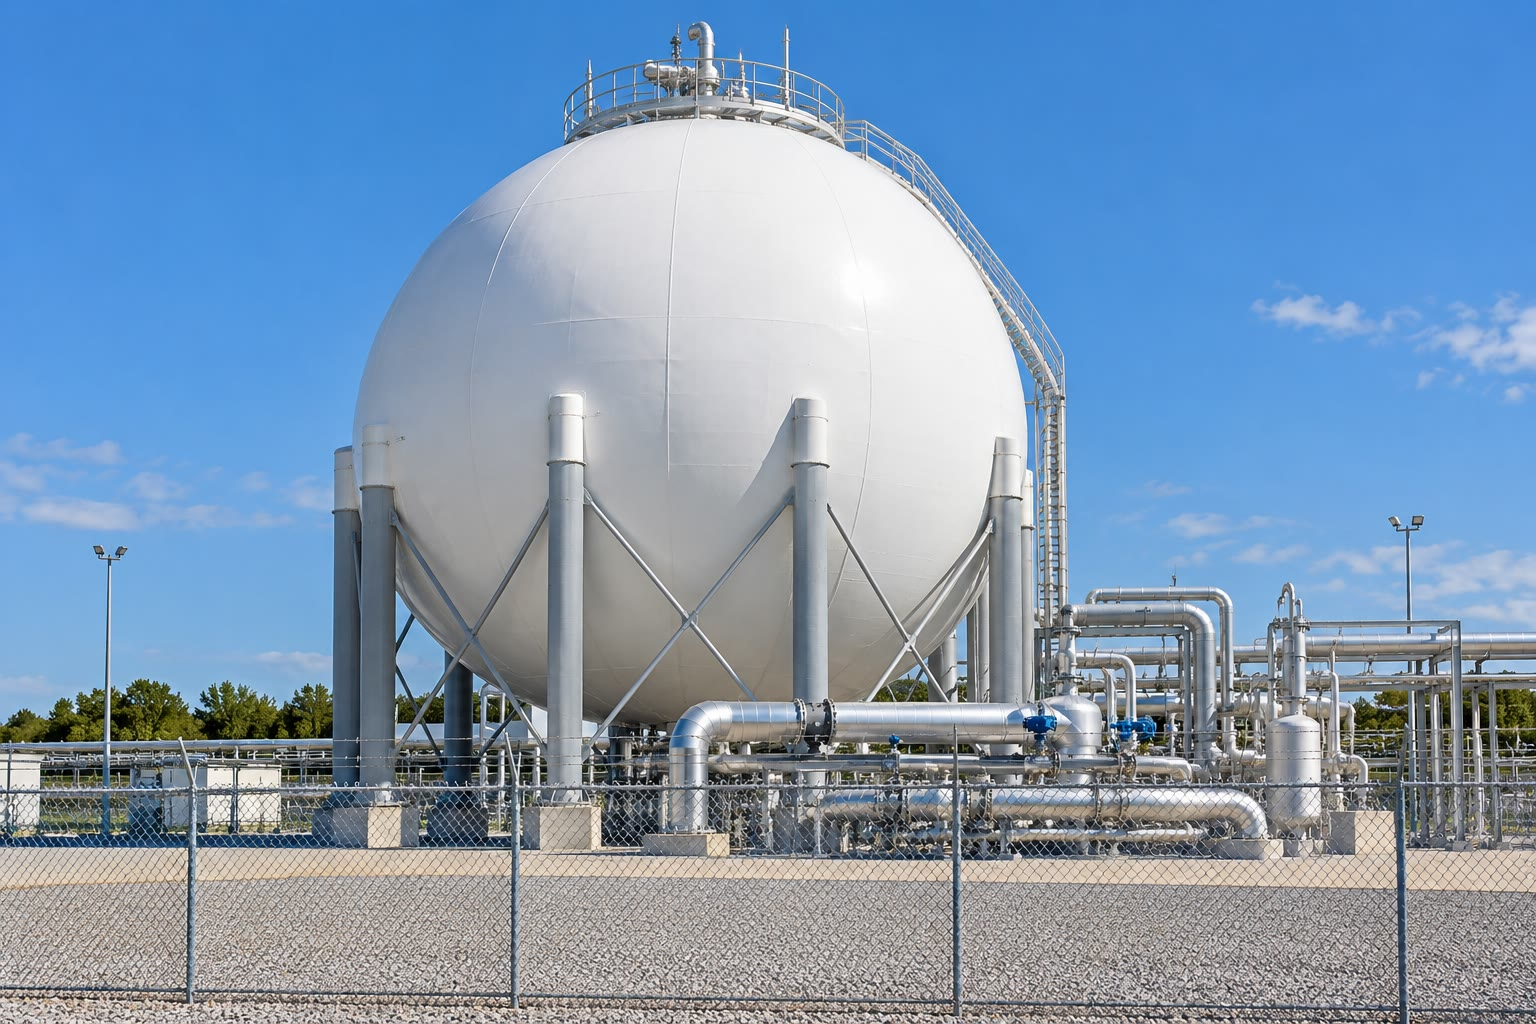
\includegraphics[width=0.6\linewidth]{images/book4/ai/b3-11-lh2-tank.jpg}

{\small A spherical tank for liquid hydrogen. At \qty{20}{K}, heat produced inside
the liquid by the slow conversion of one nuclear-spin form of hydrogen into the
other can exceed the heat that leaks in from outside.}
\end{omfigure}

\section{Heat capacities of gases}

The heat capacity at constant volume is $C_V = (\partial U/\partial T)_V$, and with
\cref{thm:b3:partition-functions:internal-energy} each kind of motion
contributes separately. Two limits govern everything.

\begin{theorem}[Equipartition theorem]\label{thm:b3:statistical-thermo-applied:equipartition}
When the energy levels of a motion are closely spaced compared with $kT$, each
term of its energy that is quadratic in a coordinate or a momentum contributes
$\frac12kT$ to the mean energy of a molecule, hence $\frac12R$ to the molar heat
capacity. This statement is the \emph{equipartition theorem}\index{equipartition theorem}.
\end{theorem}

\begin{proof}[Partial proof]
In the classical limit the sum over the states of a motion becomes an
integral, and a quadratic term $a u^2$ contributes the factor $\int\eu^{-\beta au^2}\dd u =
\sqrt{\pi/\beta a}$, proportional to $\beta^{-1/2}$. By
\cref{thm:b3:partition-functions:internal-energy}, its mean energy is
$-\partial\ln(\beta^{-1/2})/\partial\beta = 1/2\beta = \frac12kT$. That the classical integral is the
limit of the quantum sum was shown for translation and rotation in
\cref{ch:b3:partition-functions}; for vibration it follows from the next
proposition when $T \gg \theta_{\mathrm V}$.
\end{proof}

Translation has three quadratic terms ($\frac32R$); the rotation of a linear
molecule two ($R$), of a non-linear one three ($\frac32R$); each vibration two,
kinetic and potential ($R$). A linear molecule of $N$ atoms thus tends to
$C_{V,\mathrm m} = \frac52R + (3N - 5)R$ at high temperature. The limit is almost never
reached for vibrations at room temperature.

\begin{proposition}[Vibrational heat capacity]\label{prop:b3:statistical-thermo-applied:cv-vib}
A harmonic vibration of characteristic temperature $\theta_{\mathrm V}$ contributes, with
$x = \theta_{\mathrm V}/T$,
\[
  \frac{C_{V,\mathrm m}^{\mathrm V}}{R} = \frac{x^2\eu^x}{(\eu^x - 1)^2},
\]
the Einstein function, which tends to 1 when $T \gg \theta_{\mathrm V}$ and falls
exponentially, as $x^2\eu^{-x}$, when $T \ll \theta_{\mathrm V}$.
\end{proposition}

\begin{proof}
From \cref{prop:b3:partition-functions:q-vib}, $U - U(0) = R\theta_{\mathrm V}/(\eu^x - 1)$ per mole.
Differentiating with respect to $T$, with $\dd x/\dd T = -x/T$, gives
$R\theta_{\mathrm V}\eu^x(x/T)/(\eu^x - 1)^2 = Rx^2\eu^x/(\eu^x - 1)^2$. For $x \to 0$, $\eu^x - 1 \approx x$ and the
ratio tends to 1; for large $x$ it behaves as $x^2\eu^{-x}$.
\end{proof}

\begin{method}[The heat capacity of a gas from its modes]\label{met:b3:statistical-thermo-applied:cv}
\begin{enumerate}
  \item Translation: $\frac32R$, always.
  \item Rotation: $R$ (linear) or $\frac32R$ (non-linear) if $T \gg \theta_{\mathrm R}$, true for every
        gas but hydrogen above a few tens of kelvins.
  \item Vibrations: one Einstein term per \omterm{def:b3:group-theory-applied:normal-mode}{normal mode}, $\theta_{\mathrm V} = hc\tilde\nu/k$ from
        the fundamental wavenumbers; a degenerate mode counts as many times as
        its \omterm{def:b3:quantum-model-systems:degenerate}{degeneracy}.
  \item Add, and $C_{p,\mathrm m} = C_{V,\mathrm m} + R$ for an ideal gas.
\end{enumerate}
\end{method}

A motion is said to be frozen when $kT$ is small compared with its first
excitation: it then holds no energy and contributes nothing to $C_V$. The
vibration of \ce{N2} ($\theta_{\mathrm V} = \qty{3352}{K}$) is frozen at room temperature and
$C_{V,\mathrm m} = \frac52R$; that of \ce{Cl2} ($\theta_{\mathrm V} = \qty{798}{K}$) is half awake,
$C_{V,\mathrm m} = 3.07R$ at \qty{300}{K}.

\begin{omfigure}
\begin{tikzpicture}
\begin{axis}[width=0.86\linewidth, height=6.4cm, xmode=log, xmin=10, xmax=3000,
  ymin=1.3, ymax=3.9, axis lines=left, xlabel={$T$ / K}, ylabel={$C_{V,\mathrm m}/R$},
  tick label style={font=\small}, label style={font=\small},
  log ticks with fixed point, xtick={10,30,100,300,1000,3000},
  unbounded coords=jump]
\addplot[omDef, thick] table[x=T, y=N2] {figdata/out/bachelor-3-heat-capacity.dat};
\addplot[black!60, thick] table[x=T, y=Cl2] {figdata/out/bachelor-3-heat-capacity.dat};
\addplot[omThm, thick, dashed] table[x=T, y=nH2] {figdata/out/bachelor-3-heat-capacity.dat};
\addplot[omThm, thick] table[x=T, y=eH2] {figdata/out/bachelor-3-heat-capacity.dat};
\addplot[only marks, mark=*, mark size=1.6pt, omDef] table[x=T, y=N2] {figdata/out/bachelor-3-heat-capacity-janaf.dat};
\addplot[only marks, mark=square*, mark size=1.5pt, black!60] table[x=T, y=Cl2] {figdata/out/bachelor-3-heat-capacity-janaf.dat};
\draw[black!30, densely dotted] (axis cs:10,1.5) -- (axis cs:3000,1.5);
\draw[black!30, densely dotted] (axis cs:10,2.5) -- (axis cs:3000,2.5);
\draw[black!30, densely dotted] (axis cs:10,3.5) -- (axis cs:3000,3.5);
\node[font=\scriptsize, black!60, anchor=south east] at (axis cs:2900,1.5) {$\frac32$: translation};
\node[font=\scriptsize, black!60, anchor=south west] at (axis cs:10.5,2.5) {$\frac52$: + rotation};
\node[font=\scriptsize, black!60, anchor=south west] at (axis cs:10.5,3.5) {$\frac72$: + vibration};
\node[font=\scriptsize, omThm, anchor=south west] at (axis cs:60,3.6) {equilibrium \ce{H2}};
\node[font=\scriptsize, omThm, anchor=north west] at (axis cs:130,1.78) {normal \ce{H2}};
\node[font=\scriptsize, black!70, anchor=south east] at (axis cs:560,3.33) {\ce{Cl2}};
\node[font=\scriptsize, omDef, anchor=south east] at (axis cs:1000,3.0) {\ce{N2}};
\end{axis}
\end{tikzpicture}

{\small Molar heat capacity at constant volume, computed from the spectroscopic
constants (lines; \omterm{def:b3:quantum-model-systems:rotor}{rigid rotor}, harmonic vibration), with the values of the
thermochemical tables for \ce{N2} and \ce{Cl2} (points, $C_p/R - 1$). Vibration wakes up
near $\theta_{\mathrm V}/10$; above about \qty{1000}{K} the tables rise above the harmonic model,
which misses the anharmonicity. Hydrogen: the rotational contribution
of normal hydrogen (dashed, ortho and para frozen at 3:1) and of equilibrium
hydrogen (solid), which overshoots $\frac52$ because converting para into ortho
absorbs heat.}
\end{omfigure}

\section{Nuclear-spin statistics}

The two nuclei of \ce{H2} are identical fermions. Exchanging them changes the sign
of the total wavefunction (\cref{ch:b3:many-electron-atoms}); exchanging them is
the same as rotating the molecule end over end, which multiplies the rotational
wavefunction $Y_{J,M}$ by $(-1)^J$ and the nuclear-spin function by $+1$ or $-1$.

\begin{theorem}[Nuclear-spin statistics]\label{thm:b3:statistical-thermo-applied:spin-statistics}
In a homonuclear diatomic molecule whose nuclei have spin $I$, in a ground
electronic state ${}^1\Sigma_g^+$, there are $(2I+1)(I+1)$ symmetric and $(2I+1)I$
antisymmetric nuclear-spin states. For fermions (half-integer $I$) the
antisymmetric ones go with even $J$ and the symmetric ones with odd $J$; for
bosons (integer $I$) the opposite. For \ce{H2} ($I = \frac12$) even and odd levels have
spin weights 1 and 3; for \ce{D2} ($I = 1$), 6 and 3. When $I = 0$ only one parity of
$J$ exists at all: the linear \ce{CO2} molecule, with two \ce{^{16}O} nuclei and a
symmetric ground state, has only even rotational levels.
\end{theorem}

\begin{proof}[Partial proof]
The symmetry postulate (the total wavefunction is antisymmetric under the
exchange of two identical fermions, symmetric for bosons) is admitted. The
$(2I+1)^2$ products of one-nucleus spin states $|m_1\rangle|m_2\rangle$ give $2I+1$ symmetric
states with $m_1 = m_2$, and for each of the $(2I+1)2I/2$ pairs $m_1 \ne m_2$ one
symmetric and one antisymmetric combination: $(2I+1) + (2I+1)I = (2I+1)(I+1)$
symmetric and $(2I+1)I$ antisymmetric states. In a ${}^1\Sigma_g^+$ state the electronic
and vibrational functions are unchanged by the exchange, so the product of
rotational and spin functions must have the required overall sign: for
fermions, $(-1)^J \times(\text{spin symmetry}) = -1$, which pairs even $J$ with
antisymmetric spin states. For \ce{H2}: 3 symmetric, 1 antisymmetric; for \ce{D2}: 6 and
3.
\end{proof}

\begin{definition}[Ortho and para hydrogen]\label{def:b3:statistical-thermo-applied:spin-isomers}
\emph{Ortho hydrogen}\index{ortho hydrogen} is the form of \ce{H2} with the two
proton spins in a symmetric (triplet) state, which occupies only the odd
rotational levels; \emph{para hydrogen}\index{para hydrogen} the form with the
antisymmetric (singlet) spin state, which occupies only the even levels.
\end{definition}

Converting one into the other requires flipping one nuclear spin relative to
the other, which collisions with other hydrogen molecules hardly do: in pure
hydrogen the two forms behave for days as two different gases. A paramagnetic
surface, whose inhomogeneous magnetic field acts differently on the two
protons, catalyses the conversion.

\begin{proposition}[Equilibrium ortho--para ratio]\label{prop:b3:statistical-thermo-applied:ortho-para}
At equilibrium the fraction of \omterm{def:b3:statistical-thermo-applied:spin-isomers}{para hydrogen} is
\[
  x_{\mathrm{para}} = \frac{\sum_{J\,\mathrm{even}}(2J+1)\eu^{-\theta_{\mathrm R}J(J+1)/T}}
    {\sum_{J\,\mathrm{even}}(2J+1)\eu^{-\theta_{\mathrm R}J(J+1)/T} + 3\sum_{J\,\mathrm{odd}}(2J+1)\eu^{-\theta_{\mathrm R}J(J+1)/T}},
\]
which tends to 1 at 0 K and to $\frac14$ at high temperature. For \ce{D2}, the ortho form
(even $J$) tends to 1 at 0 K and to $\frac23$ at high temperature.
\end{proposition}

\begin{proof}
The \omterm{def:b3:partition-functions:boltzmann}{Boltzmann distribution} over all the states, with the spin weights of
\cref{thm:b3:statistical-thermo-applied:spin-statistics}. At 0 K only $J = 0$, which is
even, is populated. At high temperature the even and odd sums are each half
of $T/\theta_{\mathrm R}$, and the ratio is $1 : 3$; for \ce{D2}, $6 : 3$.
\end{proof}

For \ce{H2}, $\theta_{\mathrm R} = \qty{85.4}{K}$: the equilibrium mixture is half para at \qty{78}{K},
99.8\,\% para at the boiling point, \qty{20.37}{K}, and 25.07\,\% at room
temperature. Hydrogen kept at room temperature, called normal hydrogen, is
therefore a 3:1 mixture of ortho and para.

\begin{omfigure}
\begin{tikzpicture}
\begin{axis}[width=0.72\linewidth, height=5.4cm, xmin=0, xmax=300, ymin=0, ymax=1.05,
  axis lines=left, xlabel={$T$ / K}, ylabel={equilibrium fraction},
  tick label style={font=\small}, label style={font=\small}]
\addplot[omThm, thick] table[x=T, y=pH2] {figdata/out/bachelor-3-ortho-para.dat};
\addplot[omDef, thick] table[x=T, y=oD2] {figdata/out/bachelor-3-ortho-para.dat};
\draw[black!35, densely dotted] (axis cs:0,0.25) -- (axis cs:300,0.25);
\draw[black!35, densely dotted] (axis cs:0,0.6667) -- (axis cs:300,0.6667);
\node[font=\scriptsize, omThm, anchor=south west] at (axis cs:190,0.27) {para fraction of \ce{H2} $\to \frac14$};
\node[font=\scriptsize, omDef, anchor=south west] at (axis cs:120,0.69) {ortho fraction of \ce{D2} $\to \frac23$};
\end{axis}
\end{tikzpicture}

{\small Equilibrium composition of the nuclear-spin isomers against
temperature, from the rotational levels and the spin weights (\ce{H2}: 1 and 3;
\ce{D2}: 6 and 3). Both forms with even $J$ take over at low temperature.}
\end{omfigure}

The heat capacity of hydrogen shows the consequences. In normal hydrogen the
ortho and para molecules are two gases mixed in fixed proportions; each has its
own ladder of levels, starting at $J = 1$ and at $J = 0$, and its rotation freezes
separately. In equilibrium hydrogen, heating also converts para into ortho, which
absorbs energy and gives the peak of the figure above. The first measurements,
made without a catalyst, followed the normal-hydrogen curve, and it was the
interpretation of that curve as a frozen 3:1 mixture that first revealed the
two forms.

\begin{remark}
The \omterm{def:b3:partition-functions:symmetry-number}{symmetry number} of \cref{prop:b3:partition-functions:q-rot} is now justified.
At high temperature each spin state finds about half the rotational levels
allowed, so that $\sum(\text{spin weight})(2J+1)\eu^{\dots} \approx (2I+1)^2\,T/2\theta_{\mathrm R}$: the
total-spin factor $(2I+1)^2$ is left out by convention, and $\sigma = 2$ remains.
\end{remark}

\begin{definition}[Residual entropy]\label{def:b3:statistical-thermo-applied:residual-entropy}
The \emph{residual entropy}\index{residual entropy} of a crystal is the entropy it
retains as $T \to 0$ because its molecules remain frozen in one of many
arrangements of equal or almost equal energy.
\end{definition}

\begin{proposition}[Residual entropies of carbon monoxide and of ice]\label{prop:b3:statistical-thermo-applied:residual}
A crystal of $N$ molecules frozen in $W_0$ equally likely arrangements has $S_0 =
k\ln W_0$. Solid \ce{CO}, each molecule pointing either way, has $S_{0,\mathrm m} = R\ln2 =
\qty{5.76}{J.K^{-1}.mol^{-1}}$. Ice, with every oxygen bonded to two hydrogen atoms
and hydrogen-bonded to two others, has $W_0 = (3/2)^N$ and $S_{0,\mathrm m} = R\ln\frac32 =
\qty{3.37}{J.K^{-1}.mol^{-1}}$.
\end{proposition}

\begin{proof}
\cref{def:b3:partition-functions:statistical-entropy} applied at $T \to 0$.
\ce{CO}: the dipole of the molecule is so small that the orientations CO and OC
have almost the same energy, and each of $N$ molecules has two: $W_0 = 2^N$,
$S_0 = Nk\ln2$. Ice (Pauling's count): each of the $2N$ hydrogen atoms sits on an
O$\cdots$O line, near one end or the other: $2^{2N}$ arrangements. Of the 16 ways of
placing the four hydrogens around one oxygen, 6 give it exactly two near
hydrogens (a water molecule); treating the oxygens as independent, a fraction
$6/16$ of the arrangements satisfies each of them: $W_0 = 2^{2N}(6/16)^N = (3/2)^N$.
\end{proof}

The tables quote, for \ce{CO}, the \omterm{def:b3:partition-functions:statistical-entropy}{statistical entropy}
(\cref{ch:b3:partition-functions}); the calorimetric value is lower by a gap of the
order of $R\ln2$, somewhat smaller because the orientations are not quite
random. For ice, the gap between the calorimetric entropy of water vapour and
its statistical value agreed with Pauling's count when he made it in 1935,
confirming that the protons of ice are disordered. The third law,
in the form ``the entropy of a perfect crystal is zero at 0 K'', applies to the
crystals that do reach a single arrangement.

\begin{omfigure}
\begin{tikzpicture}[scale=1.15, every node/.style={transform shape}]
  \draw[black!45, dashed] (0.00,0.00) -- (1.20,0.00);
  \draw[black, thick] (0.00,0.00) -- (0.36,0.00); \node[aH, minimum size=2.2mm] at (0.36,0.00) {};
  \draw[black!45, dashed] (0.00,0.00) -- (0.00,1.20);
  \draw[black, thick] (0.00,0.00) -- (0.00,0.36); \node[aH, minimum size=2.2mm] at (0.00,0.36) {};
  \draw[black!45, dashed] (0.00,1.20) -- (1.20,1.20);
  \draw[black, thick] (0.00,1.20) -- (0.36,1.20); \node[aH, minimum size=2.2mm] at (0.36,1.20) {};
  \draw[black!45, dashed] (0.00,1.20) -- (0.00,2.40);
  \draw[black, thick] (0.00,2.40) -- (0.00,2.04); \node[aH, minimum size=2.2mm] at (0.00,2.04) {};
  \draw[black!45, dashed] (0.00,2.40) -- (1.20,2.40);
  \draw[black, thick] (1.20,2.40) -- (0.84,2.40); \node[aH, minimum size=2.2mm] at (0.84,2.40) {};
  \draw[black!45, dashed] (0.00,2.40) -- (0.00,3.60);
  \draw[black, thick] (0.00,3.60) -- (0.00,3.24); \node[aH, minimum size=2.2mm] at (0.00,3.24) {};
  \draw[black!45, dashed] (0.00,3.60) -- (1.20,3.60);
  \draw[black, thick] (1.20,3.60) -- (0.84,3.60); \node[aH, minimum size=2.2mm] at (0.84,3.60) {};
  \draw[black!45, dashed] (0.00,3.60) -- (0.00,4.20);
  \draw[black, thick] (0.00,3.60) -- (0.00,3.96); \node[aH, minimum size=2.2mm] at (0.00,3.96) {};
  \draw[black!45, dashed] (1.20,0.00) -- (2.40,0.00);
  \draw[black, thick] (1.20,0.00) -- (1.56,0.00); \node[aH, minimum size=2.2mm] at (1.56,0.00) {};
  \draw[black!45, dashed] (1.20,0.00) -- (1.20,1.20);
  \draw[black, thick] (1.20,1.20) -- (1.20,0.84); \node[aH, minimum size=2.2mm] at (1.20,0.84) {};
  \draw[black!45, dashed] (1.20,1.20) -- (2.40,1.20);
  \draw[black, thick] (2.40,1.20) -- (2.04,1.20); \node[aH, minimum size=2.2mm] at (2.04,1.20) {};
  \draw[black!45, dashed] (1.20,1.20) -- (1.20,2.40);
  \draw[black, thick] (1.20,1.20) -- (1.20,1.56); \node[aH, minimum size=2.2mm] at (1.20,1.56) {};
  \draw[black!45, dashed] (1.20,2.40) -- (2.40,2.40);
  \draw[black, thick] (1.20,2.40) -- (1.56,2.40); \node[aH, minimum size=2.2mm] at (1.56,2.40) {};
  \draw[black!45, dashed] (1.20,2.40) -- (1.20,3.60);
  \draw[black, thick] (1.20,3.60) -- (1.20,3.24); \node[aH, minimum size=2.2mm] at (1.20,3.24) {};
  \draw[black!45, dashed] (1.20,3.60) -- (2.40,3.60);
  \draw[black, thick] (2.40,3.60) -- (2.04,3.60); \node[aH, minimum size=2.2mm] at (2.04,3.60) {};
  \draw[black!45, dashed] (1.20,3.60) -- (1.20,4.20);
  \draw[black!45, dashed] (2.40,0.00) -- (3.60,0.00);
  \draw[black, thick] (3.60,0.00) -- (3.24,0.00); \node[aH, minimum size=2.2mm] at (3.24,0.00) {};
  \draw[black!45, dashed] (2.40,0.00) -- (2.40,1.20);
  \draw[black, thick] (2.40,0.00) -- (2.40,0.36); \node[aH, minimum size=2.2mm] at (2.40,0.36) {};
  \draw[black!45, dashed] (2.40,1.20) -- (3.60,1.20);
  \draw[black, thick] (2.40,1.20) -- (2.76,1.20); \node[aH, minimum size=2.2mm] at (2.76,1.20) {};
  \draw[black!45, dashed] (2.40,1.20) -- (2.40,2.40);
  \draw[black, thick] (2.40,2.40) -- (2.40,2.04); \node[aH, minimum size=2.2mm] at (2.40,2.04) {};
  \draw[black!45, dashed] (2.40,2.40) -- (3.60,2.40);
  \draw[black, thick] (3.60,2.40) -- (3.24,2.40); \node[aH, minimum size=2.2mm] at (3.24,2.40) {};
  \draw[black!45, dashed] (2.40,2.40) -- (2.40,3.60);
  \draw[black, thick] (2.40,2.40) -- (2.40,2.76); \node[aH, minimum size=2.2mm] at (2.40,2.76) {};
  \draw[black!45, dashed] (2.40,3.60) -- (3.60,3.60);
  \draw[black, thick] (2.40,3.60) -- (2.76,3.60); \node[aH, minimum size=2.2mm] at (2.76,3.60) {};
  \draw[black!45, dashed] (2.40,3.60) -- (2.40,4.20);
  \draw[black!45, dashed] (3.60,0.00) -- (4.20,0.00);
  \draw[black, thick] (3.60,0.00) -- (3.96,0.00); \node[aH, minimum size=2.2mm] at (3.96,0.00) {};
  \draw[black!45, dashed] (3.60,0.00) -- (3.60,1.20);
  \draw[black, thick] (3.60,1.20) -- (3.60,0.84); \node[aH, minimum size=2.2mm] at (3.60,0.84) {};
  \draw[black!45, dashed] (3.60,1.20) -- (4.20,1.20);
  \draw[black!45, dashed] (3.60,1.20) -- (3.60,2.40);
  \draw[black, thick] (3.60,1.20) -- (3.60,1.56); \node[aH, minimum size=2.2mm] at (3.60,1.56) {};
  \draw[black!45, dashed] (3.60,2.40) -- (4.20,2.40);
  \draw[black!45, dashed] (3.60,2.40) -- (3.60,3.60);
  \draw[black, thick] (3.60,2.40) -- (3.60,2.76); \node[aH, minimum size=2.2mm] at (3.60,2.76) {};
  \draw[black!45, dashed] (3.60,3.60) -- (4.20,3.60);
  \draw[black, thick] (3.60,3.60) -- (3.96,3.60); \node[aH, minimum size=2.2mm] at (3.96,3.60) {};
  \draw[black!45, dashed] (3.60,3.60) -- (3.60,4.20);
  \draw[black, thick] (3.60,3.60) -- (3.60,3.96); \node[aH, minimum size=2.2mm] at (3.60,3.96) {};
  \draw[black!45, dashed] (-0.60,0.00) -- (0.00,0.00);
  \draw[black!45, dashed] (-0.60,1.20) -- (0.00,1.20);
  \draw[black, thick] (0.00,1.20) -- (-0.36,1.20); \node[aH, minimum size=2.2mm] at (-0.36,1.20) {};
  \draw[black!45, dashed] (-0.60,2.40) -- (0.00,2.40);
  \draw[black, thick] (0.00,2.40) -- (-0.36,2.40); \node[aH, minimum size=2.2mm] at (-0.36,2.40) {};
  \draw[black!45, dashed] (-0.60,3.60) -- (0.00,3.60);
  \draw[black!45, dashed] (0.00,-0.60) -- (0.00,0.00);
  \draw[black!45, dashed] (1.20,-0.60) -- (1.20,0.00);
  \draw[black, thick] (1.20,0.00) -- (1.20,-0.36); \node[aH, minimum size=2.2mm] at (1.20,-0.36) {};
  \draw[black!45, dashed] (2.40,-0.60) -- (2.40,0.00);
  \draw[black, thick] (2.40,0.00) -- (2.40,-0.36); \node[aH, minimum size=2.2mm] at (2.40,-0.36) {};
  \draw[black!45, dashed] (3.60,-0.60) -- (3.60,0.00);
  \node[aO, minimum size=4mm] at (0.00,0.00) {};
  \node[aO, minimum size=4mm] at (0.00,1.20) {};
  \node[aO, minimum size=4mm] at (0.00,2.40) {};
  \node[aO, minimum size=4mm] at (0.00,3.60) {};
  \node[aO, minimum size=4mm] at (1.20,0.00) {};
  \node[aO, minimum size=4mm] at (1.20,1.20) {};
  \node[aO, minimum size=4mm] at (1.20,2.40) {};
  \node[aO, minimum size=4mm] at (1.20,3.60) {};
  \node[aO, minimum size=4mm] at (2.40,0.00) {};
  \node[aO, minimum size=4mm] at (2.40,1.20) {};
  \node[aO, minimum size=4mm] at (2.40,2.40) {};
  \node[aO, minimum size=4mm] at (2.40,3.60) {};
  \node[aO, minimum size=4mm] at (3.60,0.00) {};
  \node[aO, minimum size=4mm] at (3.60,1.20) {};
  \node[aO, minimum size=4mm] at (3.60,2.40) {};
  \node[aO, minimum size=4mm] at (3.60,3.60) {};
\end{tikzpicture}

{\small Proton disorder in ice, drawn as a flat square network (the real
network is tetrahedral): every oxygen (red) has four O$\cdots$O neighbours, one
hydrogen (white) on each line, and exactly two hydrogens close to it (the ice
rules). This is one of the $(3/2)^N$ arrangements of Pauling's count; all of them
have nearly the same energy, and freezing picks one at random.}
\end{omfigure}

\section{Equilibrium constants from partition functions}

\begin{theorem}[Equilibrium constant from partition functions]\label{thm:b3:statistical-thermo-applied:k-from-q}
For a reaction $0 = \sum_J\nu_J\mathrm J$ between ideal gases,
\[
  K^\circ = \prod_J\Bigl(\frac{q^\circ_{J,\mathrm m}}{N_A}\Bigr)^{\nu_J}\eu^{-\Delta_rE_0/RT},
\]
where $q^\circ_{J,\mathrm m}$ is the partition function of $\mathrm J$ in the standard molar volume
$V^\circ_{\mathrm m} = RT/p^\circ$, each counted from its own ground state, and $\Delta_rE_0 =
\sum\nu_JE_{0,J}$ is the molar energy of reaction at 0 K, from the ground state of
the reactants to that of the products.
\end{theorem}

\begin{proof}
By \cref{thm:b3:partition-functions:entropy}, a mole of ideal gas $\mathrm J$ at $p^\circ$ has
$G^\circ_{\mathrm m} - G_{\mathrm m}(0) = -RT\ln(q^\circ_{J,\mathrm m}/N_A)$, and $G_{\mathrm m}(0)$ is the energy $E_{0,J}$
of its ground state on a scale common to all the species. So $\Delta_rG^\circ =
\Delta_rE_0 - RT\sum_J\nu_J\ln(q^\circ_{J,\mathrm m}/N_A)$, and $\Delta_rG^\circ = -RT\ln K^\circ$ gives the
result.
\end{proof}

\begin{method}[Computing an equilibrium constant from spectroscopic data]\label{met:b3:statistical-thermo-applied:k-stat}
\begin{enumerate}
  \item For each species: $q^\circ_{\mathrm m}/N_A = (kT/p^\circ)\Lambda^{-3}\times q^{\mathrm R}q^{\mathrm V}q^{\mathrm E}$, with
        \omterm{def:b3:partition-functions:symmetry-number}{symmetry numbers} and electronic degeneracies.
  \item $\Delta_rE_0$ from dissociation energies $D_0$ (measured from the ground
        vibrational level, so zero-point energies are included) or from
        formation enthalpies at 0 K.
  \item Multiply, and check the units: $K^\circ$ is a pure number, the standard
        pressure entering through $kT/p^\circ$.
\end{enumerate}
\end{method}

\begin{example}[The dissociation of iodine]\label{ex:b3:statistical-thermo-applied:iodine}
% ledger: janaf:I.dfH0, janaf:I2g.dfH0, lev:I.2P1_2, diat:I2.we, diat:I2.wexe, diat:I2.Be, diat:I2.ae, aw:I, janaf:I.logKf.1000
For $\ce{I2(g) <=> 2 I(g)}$, $\Delta_rE_0 = D_0(\ce{I2}) = 2 \times 107.164 - 65.504 = \qty{148.824}{kJ/mol}$
from the formation enthalpies at 0 K of the thermochemical tables. At
\qty{1000}{K}: for I, $\Lambda = \qty{4.90}{pm}$, $kT/p^\circ = \qty{1.381e-25}{m^3}$, $q^{\mathrm E} = 4 +
2\eu^{-10.94} = 4.0000$ (the ${}^2P_{1/2}$ level lies \qty{7603}{cm^{-1}} up), so $q^\circ_{\mathrm m}/N_A = \num{4.69e9}$;
for \ce{I2}, $\Lambda = \qty{3.47}{pm}$, $q^{\mathrm R} = 1000/(2 \times 0.05369) = 9313$ and $q^{\mathrm V} = 3.784$, so
$q^\circ_{\mathrm m}/N_A = \num{1.17e14}$. Then $K^\circ = (4.69\times10^9)^2/(1.17\times10^{14}) \times \eu^{-17.90} =
\num{3.17e-3}$, $\log K^\circ = -2.50$; the tables give $-2.51$.
\end{example}

\begin{omfigure}
\begin{tikzpicture}
\begin{axis}[name=ki, width=0.5\linewidth, height=5.6cm, xmin=0.58, xmax=1.45, ymin=-6.5,
  ymax=1, axis lines=left, xlabel={$1000\,\mathrm K/T$}, ylabel={$\log K^\circ$},
  tick label style={font=\small}, label style={font=\small},
  title={\small $\ce{I2 <=> 2 I}$}]
\addplot[black, thick] table[x=invT, y=logK] {figdata/out/bachelor-3-equilibrium-constant-stat-i2.dat};
\addplot[only marks, mark=*, mark size=1.8pt, omThm] table[x=invT, y=logK] {figdata/out/bachelor-3-equilibrium-constant-stat-i2-janaf.dat};
\node[font=\scriptsize, anchor=north east, align=right] at (axis cs:1.43,0.8) {line: statistical\\ points: tables};
\end{axis}
\begin{axis}[at={(ki.east)}, anchor=west, xshift=1.4cm, width=0.44\linewidth, height=5.6cm,
  xmin=0, xmax=2000, ymin=0, ymax=4.4, axis lines=left, xlabel={$T$ / K},
  ylabel={$K^\circ$}, tick label style={font=\small}, label style={font=\small},
  title={\small $\ce{H2 + D2 <=> 2 HD}$}, scaled x ticks=false,
  xticklabel style={/pgf/number format/1000 sep={}}]
\addplot[omDef, thick] table[x=T, y=K] {figdata/out/bachelor-3-equilibrium-constant-stat-hd.dat};
\draw[black!35, densely dotted] (axis cs:0,4) -- (axis cs:2000,4);
\node[font=\scriptsize, anchor=north east] at (axis cs:1950,3.95) {$\sigma$ limit: 4};
\end{axis}
\end{tikzpicture}

{\small Equilibrium constants computed from partition functions. Left: the
dissociation of iodine, a straight van 't Hoff line of slope $-\Delta_rH^\circ/(R\ln10)$, with
the values of the thermochemical tables (points). Right: the exchange $\ce{H2 + D2
<=> 2 HD}$, which tends to the ratio of \omterm{def:b3:partition-functions:symmetry-number}{symmetry numbers}, 4, at high temperature
and falls below it at low temperature through the zero-point energies and the
nuclear-spin restrictions.}
\end{omfigure}

\begin{proposition}[The H$_2$ + D$_2$ exchange]\label{prop:b3:statistical-thermo-applied:hd}
For $\ce{H2 + D2 <=> 2 HD}$, $K^\circ \to 4$ at high temperature.
\end{proposition}

\begin{proof}
At high temperature the translational, rotational and vibrational factors are
$m^{3/2}$, $T/\sigma\theta_{\mathrm R} \propto \mu/\sigma$ and $T/\theta_{\mathrm V} \propto \sqrt\mu$ (the \omterm{def:b3:quantum-model-systems:oscillator}{force constant}, an
electronic property, is the same for the three molecules), and $\Delta_rE_0/RT \to 0$.
With $m_{\ce{H2}} = 2$, $m_{\ce{D2}} = 4$, $m_{\ce{HD}} = 3$ and $\mu = 1/2$, 1, $2/3$ (in units of the
proton mass, ignoring the small difference between D and 2H):
\[
  K^\circ \to \Bigl(\frac{9}{8}\Bigr)^{3/2} \times \frac{(2/3)^2/1^2}{(1/2)(1)/(2 \times 2)}
  \times \frac{2/3}{\sqrt{1/2}\sqrt1}
  = \frac{27}{16\sqrt2} \times \frac{32}{9} \times \frac{2\sqrt2}{3} = 4 .
\]
All the mass factors cancel exactly: only the \omterm{def:b3:partition-functions:symmetry-number}{symmetry numbers} remain, $\sigma_{\ce{H2}}
\sigma_{\ce{D2}}/\sigma_{\ce{HD}}^2 = 4$.
\end{proof}

At \qty{298.15}{K} the statistical constant is 3.26: the zero-point energies of \ce{H2},
\ce{D2} and HD (\qty{2170.3}{cm^{-1}}, \qty{1542.3}{cm^{-1}} and \qty{1883.7}{cm^{-1}}) give $\Delta_rE_0 =
\qty{54.8}{cm^{-1}}$, a factor $\eu^{-54.8/207.2} = 0.77$; rotation, still partly quantised for
these light molecules, also matters.

\begin{proposition}[The van 't Hoff equation recovered]\label{prop:b3:statistical-thermo-applied:vant-hoff-stat}
The statistical equilibrium constant obeys $\dfrac{\dd\ln K^\circ}{\dd T} = \dfrac{\Delta_rH^\circ}{RT^2}$.
\end{proposition}

\begin{proof}
Each $q^\circ_{J,\mathrm m}$ depends on $T$ through its levels and through $V^\circ_{\mathrm m} = RT/p^\circ$:
$\dd\ln q^\circ_{J,\mathrm m}/\dd T = (U_J - U_J(0))/RT^2 + 1/T$ per mole, by
\cref{thm:b3:partition-functions:internal-energy}. Hence $\dd\ln K^\circ/\dd T =
[\Delta_rE_0 + \sum\nu_J(U_J - U_J(0)) + \sum\nu_JRT]/RT^2 = (\Delta_rU + \Delta\nu_{\mathrm g}RT)/RT^2 =
\Delta_rH^\circ/RT^2$ for ideal gases.
\end{proof}

From the slope of the left panel of the figure, the enthalpy of dissociation of
iodine near \qty{1000}{K} is \qty{154}{kJ/mol}: $D_0$ plus the extra translational
energy of two atoms over a molecule, minus its rotational and vibrational
energy.

\section{Isotope effects}

\omterm{def:b3:rovibrational-spectroscopy:rotational-constant}{Isotopologues} have the same electronic structure, hence the same potential
energy curve and \omterm{def:b3:quantum-model-systems:oscillator}{force constants}, but different masses: their vibrational
wavenumbers, zero-point energies and partition functions differ, and so do
their equilibrium constants.

\begin{definition}[Equilibrium isotope effect, fractionation factor, $\delta$ value]\label{def:b3:statistical-thermo-applied:isotope-effect}
The \emph{equilibrium isotope effect}\index{equilibrium isotope effect} of a
reaction is the ratio $K_{\mathrm{light}}/K_{\mathrm{heavy}}$ of its equilibrium constants with the
light and the heavy isotope. The \emph{fractionation factor}\index{fractionation factor}
between two phases or compounds A and B is $\alpha_{\mathrm{A/B}} = R_{\mathrm A}/R_{\mathrm B}$, where
$R$ is the ratio of the heavy to the light isotope (for example $\ce{^{18}O}/\ce{^{16}O}$). The
\emph{$\delta$ value}\index{delta value@$\delta$ value} of a sample is $\delta = (R_{\mathrm{sample}}/R_{\mathrm{standard}}
- 1) \times 1000$, in per mil (\textperthousand).
\end{definition}

\begin{proposition}[Isotope effects from zero-point energies]\label{prop:b3:statistical-thermo-applied:zpe-isotope}
For an exchange $\ce{XH + YD <=> XD + YH}$ at temperatures where the stretching
vibrations are frozen, the dominant factor of the equilibrium constant is
\[
  K \approx \exp\Bigl(-\frac{\Delta\mathrm{ZPE}}{kT}\Bigr), \qquad
  \Delta\mathrm{ZPE} = \tfrac12hc\bigl[\tilde\nu_{\mathrm{XD}} + \tilde\nu_{\mathrm{YH}} - \tilde\nu_{\mathrm{XH}} - \tilde\nu_{\mathrm{YD}}\bigr],
\]
and $\tilde\nu_{\mathrm D} \approx \tilde\nu_{\mathrm H}/\sqrt2$ for a hydrogen bound to a heavy atom. The heavy
isotope concentrates in the stiffer bond.
\end{proposition}

\begin{proof}
\Cref{thm:b3:statistical-thermo-applied:k-from-q} with the energies measured
from the bottom of the common potential curves: $\Delta_rE_0$ is the change of
\omterm{def:b3:quantum-model-systems:oscillator}{zero-point energy}. The translational and rotational factors nearly cancel
between two exchanges of the same isotopes on heavy partners, and the
vibrational partition functions are 1 when frozen. With $\tilde\nu \propto \mu^{-1/2}$ and
$\mu_{\mathrm{XD}} \approx 2\mu_{\mathrm{XH}}$ for heavy X, $\tilde\nu_{\mathrm{XD}} = \tilde\nu_{\mathrm{XH}}/\sqrt2$, and $\Delta\mathrm{ZPE} =
\frac12hc(1 - 1/\sqrt2)(\tilde\nu_{\mathrm{YH}} - \tilde\nu_{\mathrm{XH}})$: negative, so $K > 1$, when X--H is the
stiffer bond.
\end{proof}

The same reasoning explains the fractionation of oxygen isotopes between water
and its vapour, between water and the carbonate of a shell, or between two
minerals: the \omterm{def:b3:statistical-thermo-applied:isotope-effect}{fractionation factor} tends to 1 at high temperature (as
$K_{\mathrm{HD}}$ tends to its symmetry limit) and departs from 1 as the temperature
falls. Measured as $\delta$ values, it is a thermometer: the $\delta^{18}$O of the carbonate
of fossil shells records the temperature of the water in which they grew, and
that of the ice of polar cores the temperature of the clouds that formed its
snow.

\begin{inthelab}[An ortho--para converter]
A hydrogen liquefier cools the gas in stages, and between the stages passes it
through beds of a paramagnetic catalyst, typically hydrated iron(III) oxide.
The conversion heat is then removed at each temperature by the refrigerator,
and the liquid that reaches the tank is close to its equilibrium composition,
almost entirely para. Without the catalyst, the heat of conversion would be
released in the tank.
\end{inthelab}

\begin{safety}{\ghs[0.8cm]{GHS02}\ghs[0.8cm]{GHS04}}
% ledger: ghs:H2
Hydrogen: an extremely flammable gas, stored under pressure or as a cryogenic
liquid. It forms explosive mixtures with air over a very wide range and burns
with an almost invisible flame; the liquid causes cold burns and its vapour
displaces air.
\end{safety}

\begin{history}[The two hydrogens, 1927--1929]
Werner Heisenberg and Friedrich Hund predicted in 1927 that hydrogen molecules
should exist in two forms differing by their nuclear spins, and David Dennison
showed the same year that the puzzling heat capacity of hydrogen measured
below room temperature was that of a 3:1 mixture of the two, frozen in its
room-temperature composition. In 1929 Karl Friedrich Bonhoeffer and Paul
Harteck adsorbed hydrogen on charcoal at liquid-air temperature, desorbed
almost pure \omterm{def:b3:statistical-thermo-applied:spin-isomers}{para hydrogen}, recognised by its different thermal conductivity,
and found that it changed back into the normal mixture only very slowly.
\end{history}

\section{Exercises}

\begin{exercise}[$\star$]\label{exo:b3:statistical-thermo-applied:1}
Give the high-temperature limit of $C_{V,\mathrm m}$ of \ce{CO2} (linear, 3 atoms), and say
which contributions are still frozen at room temperature.
\end{exercise}

\begin{exercise}[$\star$]\label{exo:b3:statistical-thermo-applied:2}
Evaluate the Einstein function at $T = \theta_{\mathrm V}$ and at $T = \theta_{\mathrm V}/10$.
\end{exercise}

\begin{exercise}[$\star$]\label{exo:b3:statistical-thermo-applied:3}
% ledger: diat:H2.Be, diat:H2.ae
With $\theta_{\mathrm R} = \qty{85.35}{K}$ for \ce{H2}, compute the equilibrium para fraction at
\qty{20}{K} (only $J = 0$ and $J = 1$ matter) and at \qty{77}{K} ($J \le 3$).
\end{exercise}

\begin{exercise}[$\star$]\label{exo:b3:statistical-thermo-applied:4}
Explain why deuterium (nuclear spin 1) gives ortho:para weights $6 : 3$, which
form is stable at 0 K, and what the ratio is at room temperature.
\end{exercise}

\begin{exercise}[$\star\star$]\label{exo:b3:statistical-thermo-applied:5}
% ledger: diat:H2.we, diat:H2.wexe, diat:D2.we, diat:D2.wexe, diat:HD.we, diat:HD.wexe
The zero-point energies of \ce{H2}, \ce{D2} and HD are 2170.3, 1542.3 and
\qty{1883.7}{cm^{-1}}. Compute $\Delta_rE_0$ for $\ce{H2 + D2 <=> 2 HD}$ and the factor $\eu^{-\Delta_rE_0/RT}$ at
\qty{298.15}{K}. Compare $4\eu^{-\Delta_rE_0/RT}$ with the full statistical value, 3.26.
\end{exercise}

\begin{exercise}[$\star\star$]\label{exo:b3:statistical-thermo-applied:6}
Estimate the \omterm{def:b3:statistical-thermo-applied:residual-entropy}{residual entropy} of a crystal of \ce{N2O} (linear NNO, which can
point either way) and of \ce{CH3D} (which can place its D on any of four
positions).
\end{exercise}

\begin{exercise}[$\star\star$]\label{exo:b3:statistical-thermo-applied:7}
% ledger: diat:Cl2.we, diat:Cl2.wexe, janaf:Cl2.Cp.300
Compute $C_{p,\mathrm m}$ of \ce{Cl2} at \qty{300}{K} from $\theta_{\mathrm V} = \qty{797.6}{K}$ and compare with the
tabulated \qty{33.981}{J.K^{-1}.mol^{-1}}.
\end{exercise}

\begin{exercise}[$\star\star$]\label{exo:b3:statistical-thermo-applied:8}
% ledger: diat:I2.we, diat:I2.wexe
Compute the vibrational heat capacity of \ce{I2} ($\theta_{\mathrm V} = \qty{306.9}{K}$) at
\qty{298.15}{K}, as a fraction of its equipartition value.
\end{exercise}

\begin{exercise}[$\star\star$]\label{exo:b3:statistical-thermo-applied:9}
A water sample A has $\delta^{18}\mathrm O = -10.0$\,\textperthousand\ and a sample B
$+2.0$\,\textperthousand\ on the same scale. Which is richer in \ce{^{18}O}? Compute the
\omterm{def:b3:statistical-thermo-applied:isotope-effect}{fractionation factor} $\alpha_{\mathrm{A/B}}$.
\end{exercise}

\begin{exercise}[$\star\star\star$]\label{exo:b3:statistical-thermo-applied:10}
In the exchange $\ce{XH + YD <=> XD + YH}$ (data of the exercise), $\tilde\nu_{\mathrm{XH}} =
\qty{3000}{cm^{-1}}$ and $\tilde\nu_{\mathrm{YH}} = \qty{2000}{cm^{-1}}$, with X and Y heavy. Estimate $K$ at
\qty{298.15}{K} and say where the deuterium goes.
\end{exercise}

\begin{exercise}[$\star\star\star$]\label{exo:b3:statistical-thermo-applied:11}
% ledger: janaf:I.dfH0, janaf:I2g.dfH0, lev:I.2P1_2, diat:I2.we, diat:I2.wexe, diat:I2.Be, diat:I2.ae, aw:I
The statistical constants of $\ce{I2 <=> 2 I}$ are $\log K^\circ = -3.392$ at \qty{900}{K} and
$-1.766$ at \qty{1100}{K}. Deduce the mean $\Delta_rH^\circ$ over the interval and explain
why it exceeds $D_0 = \qty{148.8}{kJ/mol}$.
\end{exercise}

\begin{exercise}[$\star\star\star$]\label{exo:b3:statistical-thermo-applied:12}
For \omterm{def:b3:statistical-thermo-applied:spin-isomers}{para hydrogen} at low temperature only $J = 0$ and $J = 2$ matter. Show that
its rotational heat capacity is $C/R = 5x^2\eu^{-x}/(1 + 5\eu^{-x})^2$ with $x = 6\theta_{\mathrm R}/T$, and
evaluate it at \qty{100}{K} ($\theta_{\mathrm R} = \qty{85.35}{K}$).
\end{exercise}

\section{Problem: Storing Liquid Hydrogen}

\begin{problem}[{Weekend problem --- storing liquid hydrogen: the two
nuclear-spin forms, the heat of their conversion, the boil-off it causes and
the catalyst that prevents it}]
\label{pb:b3:statistical-thermo-applied:1}
% ledger: diat:H2.Be, diat:H2.ae, diat:H2.De, hvap:nH2, tb:nH2, aw:H
Hydrogen is liquefied at its boiling point, \qty{20.37}{K} under \qty{1.01325}{bar}, where its
enthalpy of vaporisation is \qty{0.905}{kJ/mol}. Rotational levels: $F(J) = B_0J(J+1) -
D J^2(J+1)^2$ with $B_0 = \qty{59.322}{cm^{-1}}$ and $D = \qty{0.0471}{cm^{-1}}$ ($\theta_{\mathrm R} = \qty{85.35}{K}$).
Molar mass \qty{2.016}{g/mol}. The uncatalysed ortho $\to$ para conversion in the liquid
is taken first-order, $k = \qty{0.0114}{h^{-1}}$ (data of the problem).

\medskip\noindent\textbf{Part I --- The two forms.}
\begin{enumerate}
  \item How many nuclear-spin states does a pair of protons have? How many are
        symmetric under exchange, how many antisymmetric?
  \item Which spin states go with even $J$, which with odd $J$, and why?
  \item Give the spin weights of the even and odd levels.
  \item Show that the ortho:para ratio of hydrogen at room temperature is 3:1.
  \item Compute the energy of $J = 1$ above $J = 0$, in \unit{cm^{-1}} and in
        \unit{kJ/mol}.
  \item Compute the equilibrium para fraction at \qty{20.37}{K}.
  \item The equilibrium mixture is half para at about \qty{78}{K}. Why is this
        temperature close to $\theta_{\mathrm R}$?
\end{enumerate}

\medskip\noindent\textbf{Part II --- The heat of conversion.}
\begin{enumerate}[resume]
  \item What is the ortho fraction of freshly liquefied hydrogen without a
        catalyst? Why does it not change during liquefaction?
  \item Compute the heat released when a mole of it reaches equilibrium at
        \qty{20.37}{K}.
  \item Express it per kilogram.
  \item Express the enthalpy of vaporisation per kilogram.
  \item Compare the two.
  \item Why can a better insulation of the tank not remove this heat?
\end{enumerate}

\medskip\noindent\textbf{Part III --- Boil-off.}
\begin{enumerate}[resume]
  \item Give the ortho fraction after a time $t$ in the tank.
  \item Compute it after \qty{24}{h}.
  \item Compute the heat released per mole of liquid in the first \qty{24}{h}.
  \item What fraction of the liquid would this heat evaporate?
  \item Repeat for a week. Why does this simple estimate overstate the loss?
  \item Compute the half-life of the conversion.
\end{enumerate}

\medskip\noindent\textbf{Part IV --- The catalyst and the heat capacity.}
\begin{enumerate}[resume]
  \item Where, in a liquefier, should the conversion take place, and why?
  \item Is normal hydrogen at \qty{300}{K} at ortho--para equilibrium?
  \item Why do normal and equilibrium hydrogen have different heat capacities
        between about 30 and \qty{200}{K}?
  \item Read on the heat-capacity figure the maximum of $C_{V,\mathrm m}/R$ of equilibrium
        hydrogen, and explain why it exceeds $\frac52$.
  \item What is $C_{V,\mathrm m}/R$ of normal hydrogen at \qty{50}{K}?
  \item State the result: the ratio of the heat of conversion of normal hydrogen
        to its enthalpy of vaporisation, and its meaning for the tank.
\end{enumerate}
\end{problem}
